\chapter{Study of Particle Multiplicity of Cosmic Ray Events using
  2\,m\,$\times$\,2\,m Resistive Plate Chamber Stack at IICHEP-Madurai}

One of the main goals of the INO Project is to collaborate with Indian
Industries in order to streamline the production and the procurement
of variouns components as well as the RPC detectors. Transfer of
technologies and experiences in between industries and research teams
is the key aspect of this effort.
An experimental setup consisting of 12 layers of glass Resistive Plate
Chambers (RPCs) of size 2\,m\,$\times$\,2\,m has been built at
IICHEP-Madurai (\ang{9;56;14.5}\,N \ang{78;00;47.9}\,E, on the surface)
to study the long term performance and stability of RPCs produced on
large scale in Indian industry. This setup has been collecting data
triggered by the passage of charged particles. The data is analysised
to understand the behaviour of the RPCs as well as the electronics
used to run and collect data from the setup. The data is also utilised
to gain knowledge of the cosmic ray muons reaching the surface of
earth. The measurement of the multiplicity of charged particles due to
cosmic ray interactions are presented here. The results are compared
with different hadronic models of the CORSIKA simulation. The data
collected near magnetic equator gives us vital information regarding
the capabilities of the simulation packages. As the current
experimental setup is located within 81\,km from INO-Site, in depth
analysis of this data gives also improves the the packages which are
being used in the Monte-Carlo simulations for this project.

\section{Aim of the Study ****}

The upper atmoshere of the Earth gets a large dosage of exposure of
high energy primary cosmic rays originating in outer space. These
primary cosmic rays consist of mostly protons with a smaller fraction
of higher \mbox{Z-Nuclei} elements\cite{cosmic1}. The angular
distributions of the primary cosmic rays are more or less isotropic
at the top of the earth atmosphere. The energy spectrum of the primary
cosmic rays follows the power-law spectrum, $dN/dE \propto E^{-\gamma}$,
where power-law parameter, $\gamma \sim $ 2.7. The shower of secondary
particles consisting mainly of
\mbox{pions $\left(\pi^{\pm}/\pi^0\right)$} and
\mbox{kaons $\left(K^{\pm}\right)$} which are produced due the
interactions of primary cosmic rays with atmospheric nuclei.
The neutral pions mainly decay via electro-magnetic interactions,
$\pi^0 \rightarrow \gamma+\gamma$ whereas the charged pions decay to
muons and neutrinos via weak-interactions,
$\pi^+ \rightarrow \mu^+ + \nu_{\mu}$ and
$\pi^- \rightarrow \mu^- + \bar{\nu}_{\mu}$. The kaons also decay to
muons and neutrino and to pions in different branching fractions.
Most of the pions and kaons decay in flight and do not reach the
earth's surface.
The $\gamma$, $e^{\pm}$ do not reach the detector directly as they
interact with the roof of the laboratory and generate electromagnetic
showers. Only a small fraction of resultant muons decay into
electrons and neutrinos, 
$\mu^+ \rightarrow e^+ + \nu_{e} + \bar{\nu}_{\mu}$ and 
$\mu^- \rightarrow e^- + \bar{\nu}_{e} + \nu_{\mu}$. Thus, muons are the
most abundant charged particle from cosmic ray showers detected in the
present setup. These atmospheric muons are produced at high altitude
(average height of 20\,km) in the atmosphere and lose almost 2\,GeV
energy via ionisation loss in the air before reaching the ground. The 
density of charged particles (mainly muons) per unit surface area at
the earth's surface depends on the composition of primary cosmic ray,
power-law parameter ($\gamma$) as well as the model of hadronic
interactions at high energy which is not accessible in the laboratory.

The principal aim of this work is to observe the charged-particle
multiplicity in the atmospheric muon data collected
at IICHEP, Madurai and compare it with the air shower simulation.

In this study, the detector setup has been described in
the Section~\ref{sec:detectorA}. The Monte-Carlo simulation techniques
used to study the multiplicity has been explained in
Section~\ref{sec:montecarlo}, where primary cosmic ray interactions
are simulated using the CORSIKA Package\cite{corsika763} and
interactions of the particle with detector material is simulated
using the GEANT4 toolkit\cite{geant4}.


\section{Detector Setup} \label{sec:detectorA}
The RPC stack operational at IICHEP, Madurai consisting of 12 RPCs
stacked horizontally with an inter-layer gap of 16\,cm is shown in
Figure~\ref{fig:stack} where the $X$-axis of the detector is making an
angle of $-10^\circ$ with the geographic south.
\begin{figure}[h]
  \centering
  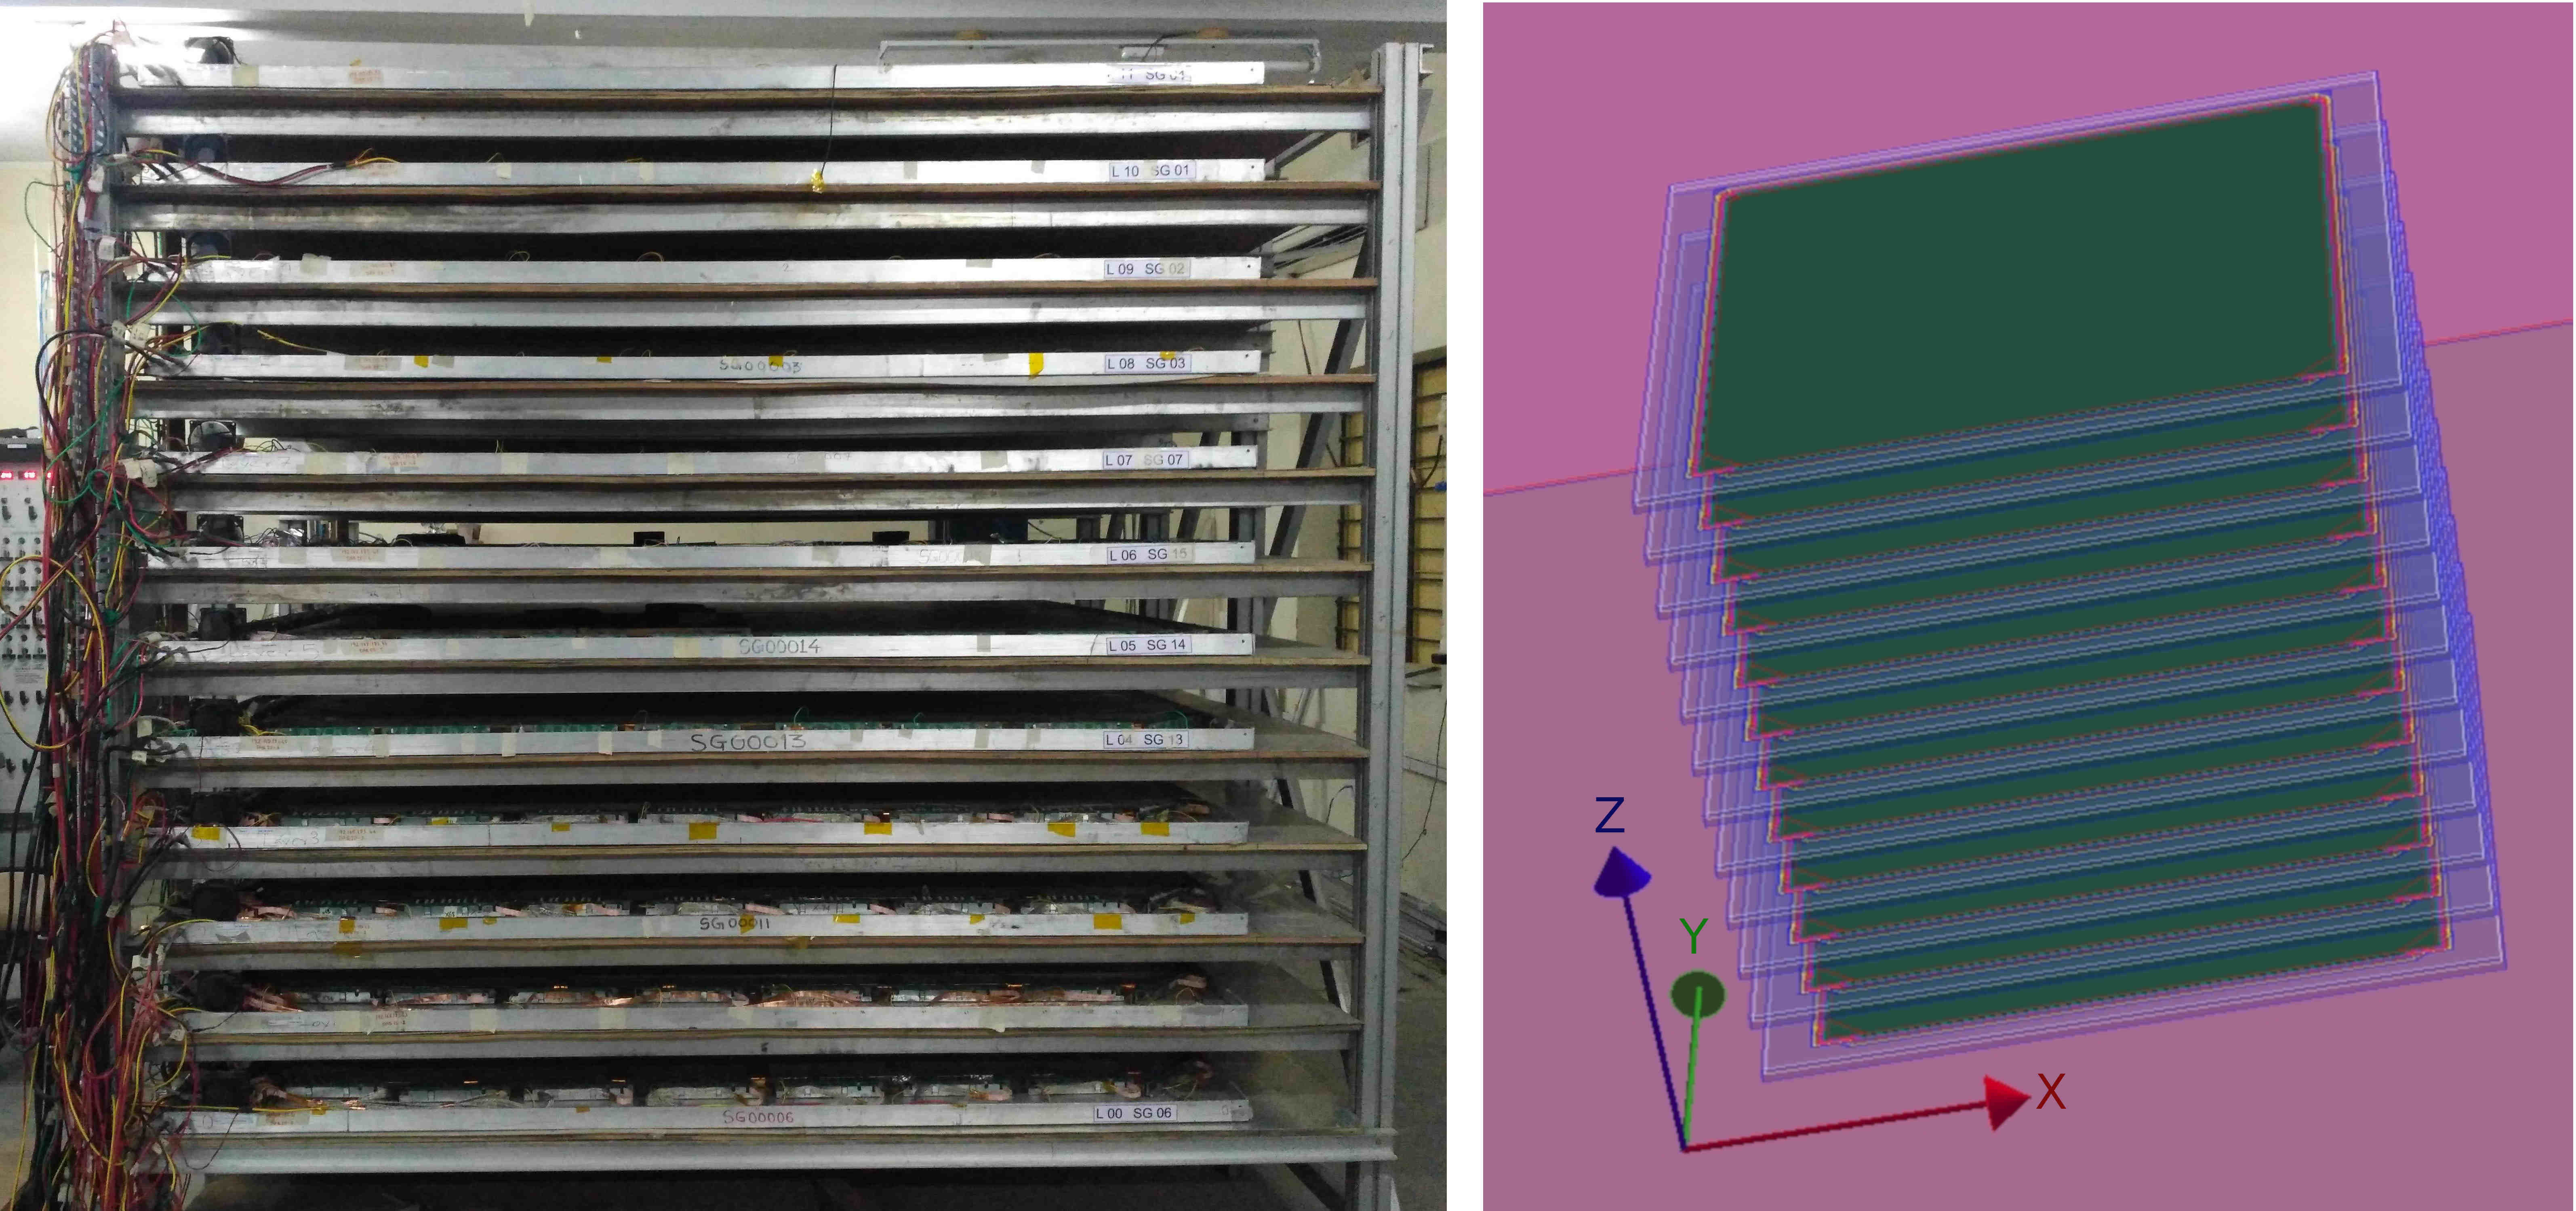
\includegraphics[width=0.99\linewidth]{ABlockStackiDAQ_new.jpg} 
  \caption{The detector stack with 12 layers of RPCs where the
    $X$-axis of the detector is making an angle of $-10^\circ$ with
    the geographic south, (left) experimental setup and (right) Geant4
    detector geometry of stack.}
  \label{fig:stack}
\end{figure}
An RPC gap is made of two glass electrodes of thickness 3\,mm with
a gap of 2\,mm between them. Uniform gap between these two electrodes
is maintained using a array of 2\,mm thick poly-carbonate buttons.
The glass gap is sealed on the outer edges to make it air-tight.
A non-flammable mixture of gas is continuously
flown inside the glass gaps through strategically placed nozzled.
This mixture of gasses serves as the active medium of the detector.
The RPCs are operated in avalanche mode. In this case, the mixture of
gases consists of R134a (95.2\%), iso-C$_4$H$_{10}$ (4.2\%) and
SF$_6$ (0.3\%). Both the outer surfaces of the glass gap are coated
with a thin layer of graphite. The RPCs are operated by applying
a differential supply of $\pm$\,5\,kV to the graphite layers to
achieve the desired electric field. The target gas inside the RPCs get
ionised by the transit of charged particles. This ionisation eventually
evloves into a avalanche in the presence of the high electric field
between the glass elctrodes. The avalanche in the RPCs induces
signals in the two orthogonal pickup panels placed on both sides of
the glass gaps labeled as X-side and Y-side. The pickup
panels are made of parallel copper strips of width 28\,mm with 2\,mm
gap between two consecutive strips. The RPCs used in this detector
stack are of the size of 1790\,mm\,$\times$\,1890\,mm. There are
60 strips on the X side and 63 strips on the Y side for each layer.

The induced signals from the pickup strips are amplified and
discriminated by a charge sensitive NINO\cite{nino} front-end
amplifier-discriminator board. Only in layer 11 (topmost layer),
ANUSPARSH front-end ASIC\cite{anusp} which is a CMOS, 8-channel,
high speed, low power amplifier-discriminator designed for
avalanche mode of operation for RPCs is used to study its performance.
The discriminated signals from these front-end boards are passed
to the FPGA-based RPCDAQ-board. The individual signals from every 
8$^{th}$ strips are \emph{OR}ed to get pre-trigger signals (S0 to S7).
The 1-fold (S0+S1+...S7), 2-fold (S0.S1+S1.S2+..S6.S7),
3-fold (S0.S1.S2+....S5.S6.S7) and 4-fold
(S0.S1.S2.S3+....S4.S5.S6.S7) signals created by RPCDAQ are passed
to the Trigger system module via Signal Router Board. The Global
Trigger is generated by Global Trigger Logic Board based (GTLB)
on X- or Y-plane with at least one strip hit within
100\,ns coincidence window. The coincidence is done for X and Y plane
independently and the final trigger can be generated by GTLB by OR
of Trigger in X- or Y-plane. The event signals in the RPCDAQ board
stretched to 1\,$\mu$s to overcome trigger latency from Trigger System
to RPCDAQ. Based on the arrival of trigger signals to RPCDAQ,
the event signals are latched and sent to the Data Concentrator
and Event Builder via Network Switch. The flow of signals from the
RPCs to the Back-End is shown in Figure~\ref{fig:sigflow}.
\begin{figure}[h]
  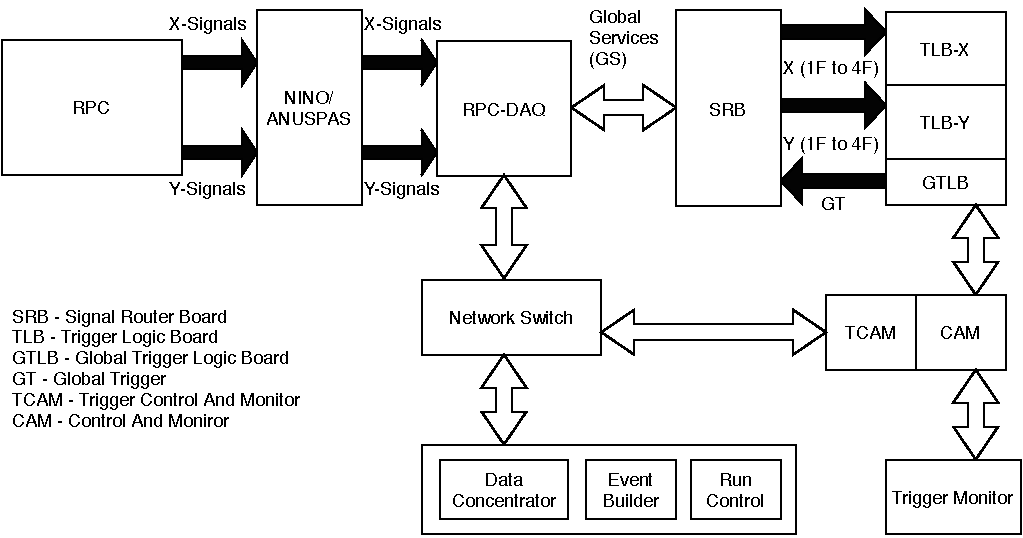
\includegraphics[width=1.0\linewidth]{DAQSchemeNewElectronics.pdf} 
  \caption{Signal flow from RPC to Back-End.}
  \label{fig:sigflow}
\end{figure}
The detailed description of signal processing and the Data Acquisition
system (DAQ) can be found in \cite{elec1}. The 1-Fold signals
from layers 4, 5, 6 and 7 are used as trigger to record the cosmic
events used in the present work.

Although the coincidence window is 100\,ns, event as well as noise
signals in a time window of 800\,ns after generation of the trigger
are also recorded due to stretching of the event latch. An event
typically contains strip hit and timing information of an event.
The strip hit is basically one logic bit per strip indicating
the signal in that strip is above the threshold value for each strip.
The timing data is consists of 16 time signal for each layer where
each TDC channel records time signals coming from every alternating
8$^{th}$ strips on one side of the layer.
The cosmic events recorded in the detector for the total observation
period of $\sim$\,17\,days between August 23, 2017, to September 8,
2017, with a trigger rate of $\sim$230\,Hz are used for the analysis.


\section{Monte-Carlo Simulation} \label{sec:montecarlo}
The Monte-Carlo Simulation for this study has been executed in
two stages. The Extensive Air Shower (EAS) has been simulated
by the CORSIKA simulation package\cite{corsika763}. The information
of daughter particles generated by the EAS at the earth's surface
level has been extracted and used as the input data to the detector
simulation. The detector simulation has been executed with the help
of the GEANT4 toolkit\cite{geant4}.

\subsection{Extensive Air Shower}
The CORSIKA (COsmic Ray SImulations for KAscade) is developed to study
the evolution of the EAS in the atmosphere created by primary cosmic
ray. Though the CORSIKA has been developed initially for a specific
experiment, this package is now developed into a tool that is used
by many groups studying cosmic rays and EAS.
In the current study, existing extrapolations of hadronic interaction
models of high energy particles in the EAS are based on
various theoretical models, which has large uncertainties.
The current experimental data at the collider experiments is
insufficient to verify the extrapolation of the hadronic interactions
at very high energies. In the CORSIKA package, the several different
hadronic interaction models are available. In this study, for
simulating the behaviour of hadrons for higher energy range,
the QGSJET (Quark Gluon String model with JETs)\cite{corsika763} has
been adopted and for the low energy range (less than 80\,GeV in
laboratory frame), the GHEISHA model has been used.

In this study, the primary cosmic ray shower has been simulated using
the CORSIKA(v7.6300) Package. The energy of the primary rays in the
CORSIKA is generated using the power-law spectrum, $E^{-2.7}$, within
the energy range of \mbox{$10$--$10^{6}$\,GeV} for different primaries
(H, He, C, O, Si and Fe). The zenith and azimuth angle of the primary
cosmic particles are generated uniformly within the range of
\mbox{$0$--$85^\circ$} and \mbox{$0$--$360^\circ$}, respectively. The
rigidity cutoff due to the earth's magnetic field has been implemented
as per the location of the detector. The minimum energy cutoffs for
secondary hadrons, muons, electrons and photons in the simulation are
kept at 50\,MeV, 10\,MeV, 1\,MeV and 1\,MeV, respectively. These cutoff
values are much smaller than the minimum momentum cutoff for
the charged particles in the vertical direction,
\mbox{$\sim 70$\,MeV}, which is mainly due to 15\,cm of concrete
roof of the building where the detector is placed. The momentum
spectra of secondary charged particles generated by the CORSIKA
simulation is shown in the Figure~\ref{fig:momin}.
\begin{figure}[h]
  \centering
  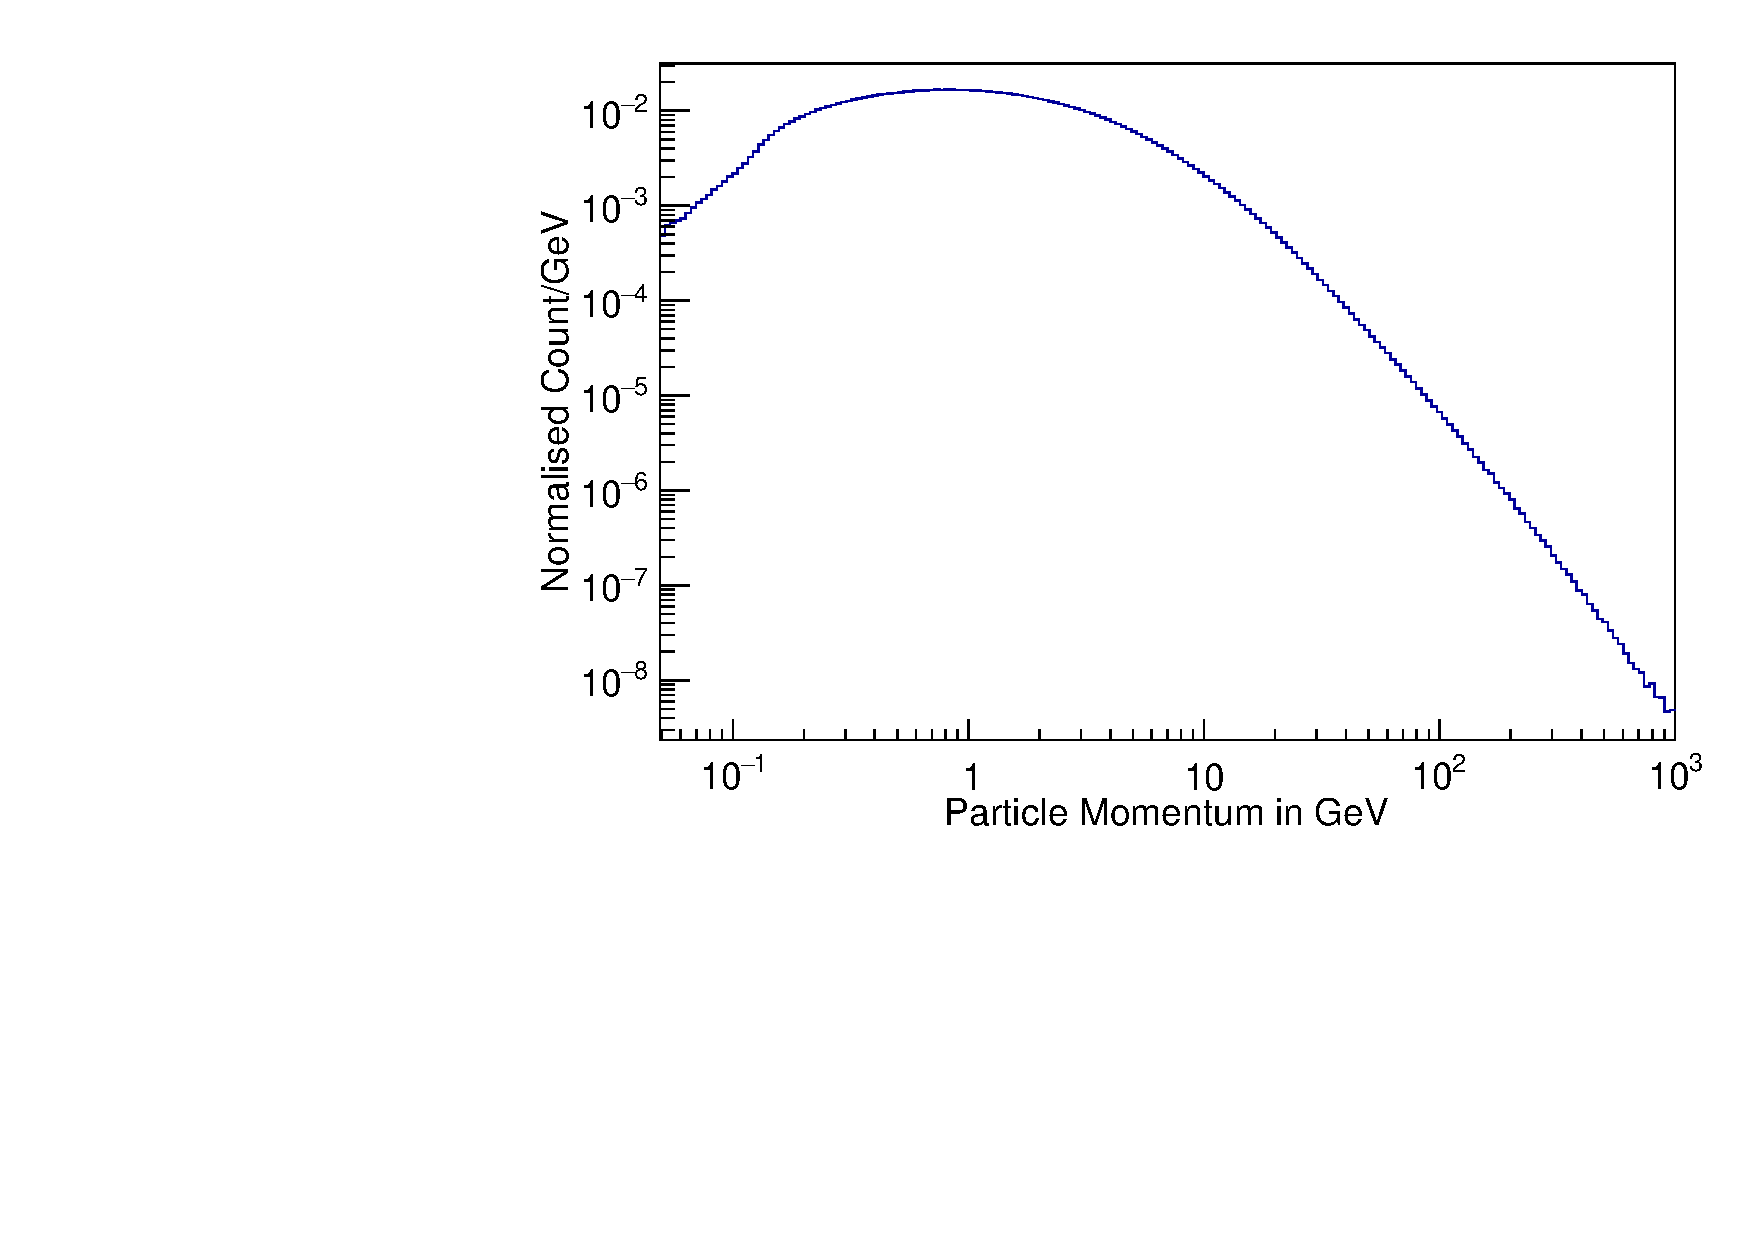
\includegraphics[width=0.6\linewidth]{momin_reco_1.pdf} 
  \caption{CORSIKA generated momentum of charged particle at observation level.}
  \label{fig:momin}
\end{figure}

The secondary particles generated by the CORSIKA which are reaching
the observation surface are provided as an input to the detector
simulation. The observation plane has been divided
into squares of the size of 2\,m\,$\times$\,2\,m which is shown in the
Figure~\ref{fig:eas}.
\begin{figure}[h]
  \centering
  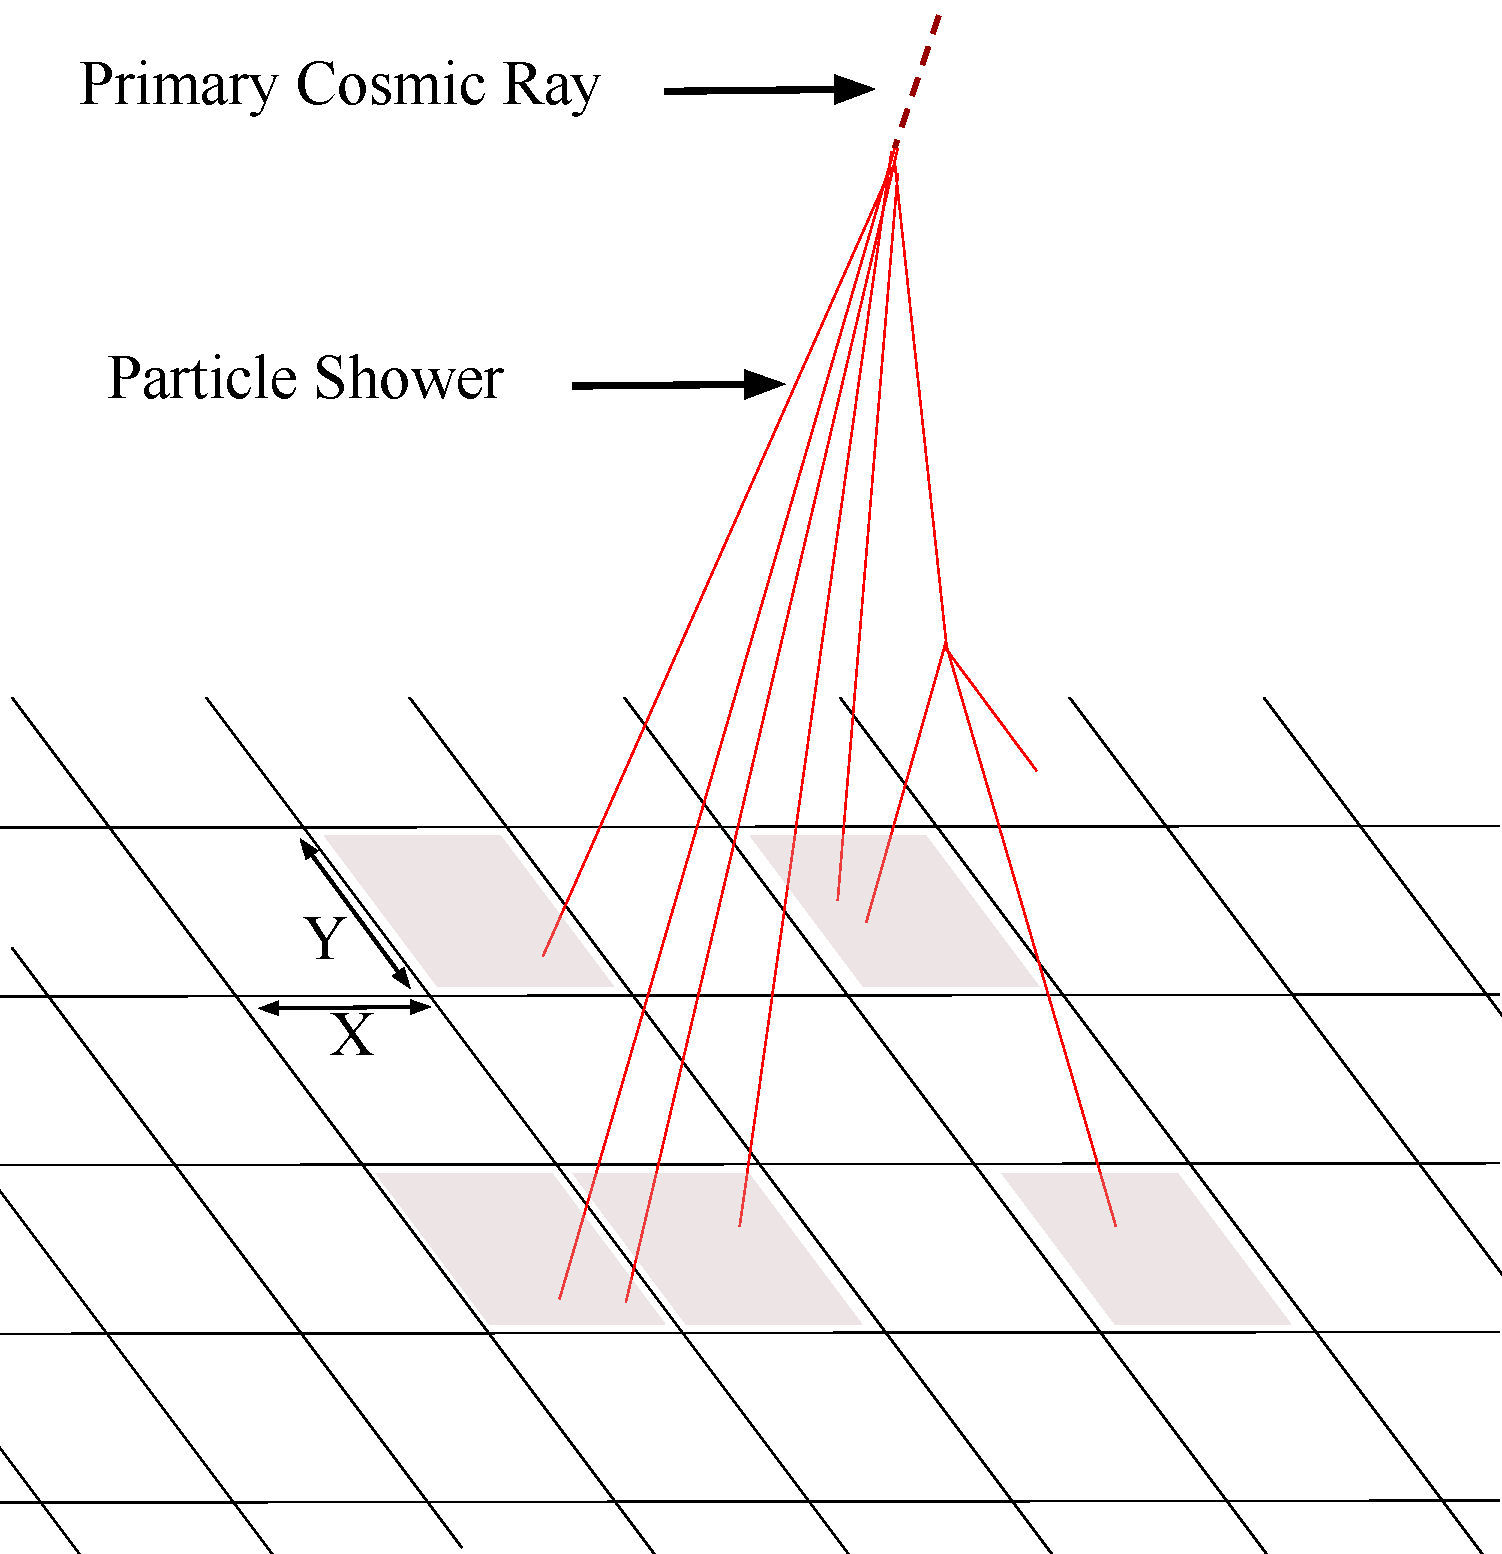
\includegraphics[width=0.6\linewidth]{EAS.pdf} 
  \caption{Shower of particles initiated by primary cosmic ray
    reaching observation surface.}
  \label{fig:eas}
\end{figure}
An event is formed using the information of the particle(s) reaching
to each of these rectangles shown as shaded region in the
Figure~\ref{fig:eas}.


\subsection{Detector Simulation}
The detector simulation has been accomplished using the
GEANT4(v4-10.0.2) toolkit. The events generated in the CORSIKA
simulation are propagated event-by-event in the detector simulation.
A realistic depiction of the detector setup including the building
where the detector is housed has been constructed in the GEANT4
environment. The materials of the various detector components and
the laboratory building are chosen based on the knowledge of the
setup. The uncertainty of the material budget is taken as a systematic
error. The physics processes of matter-particle interactions 
like electromagnetic, ionisation, decay and hadronic interactions,
which are available within the GEANT4 toolkit are considered in the
simulation.

The detector parameters like efficiency, noise, strip multiplicity,
resolution, etc. are calculated from the data gathered in the
detector. A detailed study of these parameters are presented in
\cite{pethu1}. The efficiency map, noise and strip multiplicity
profile for one of the RPCs in the stack is shown in the
Figure~\ref{fig:layer2y}.
\begin{figure}[h]
  \centering
  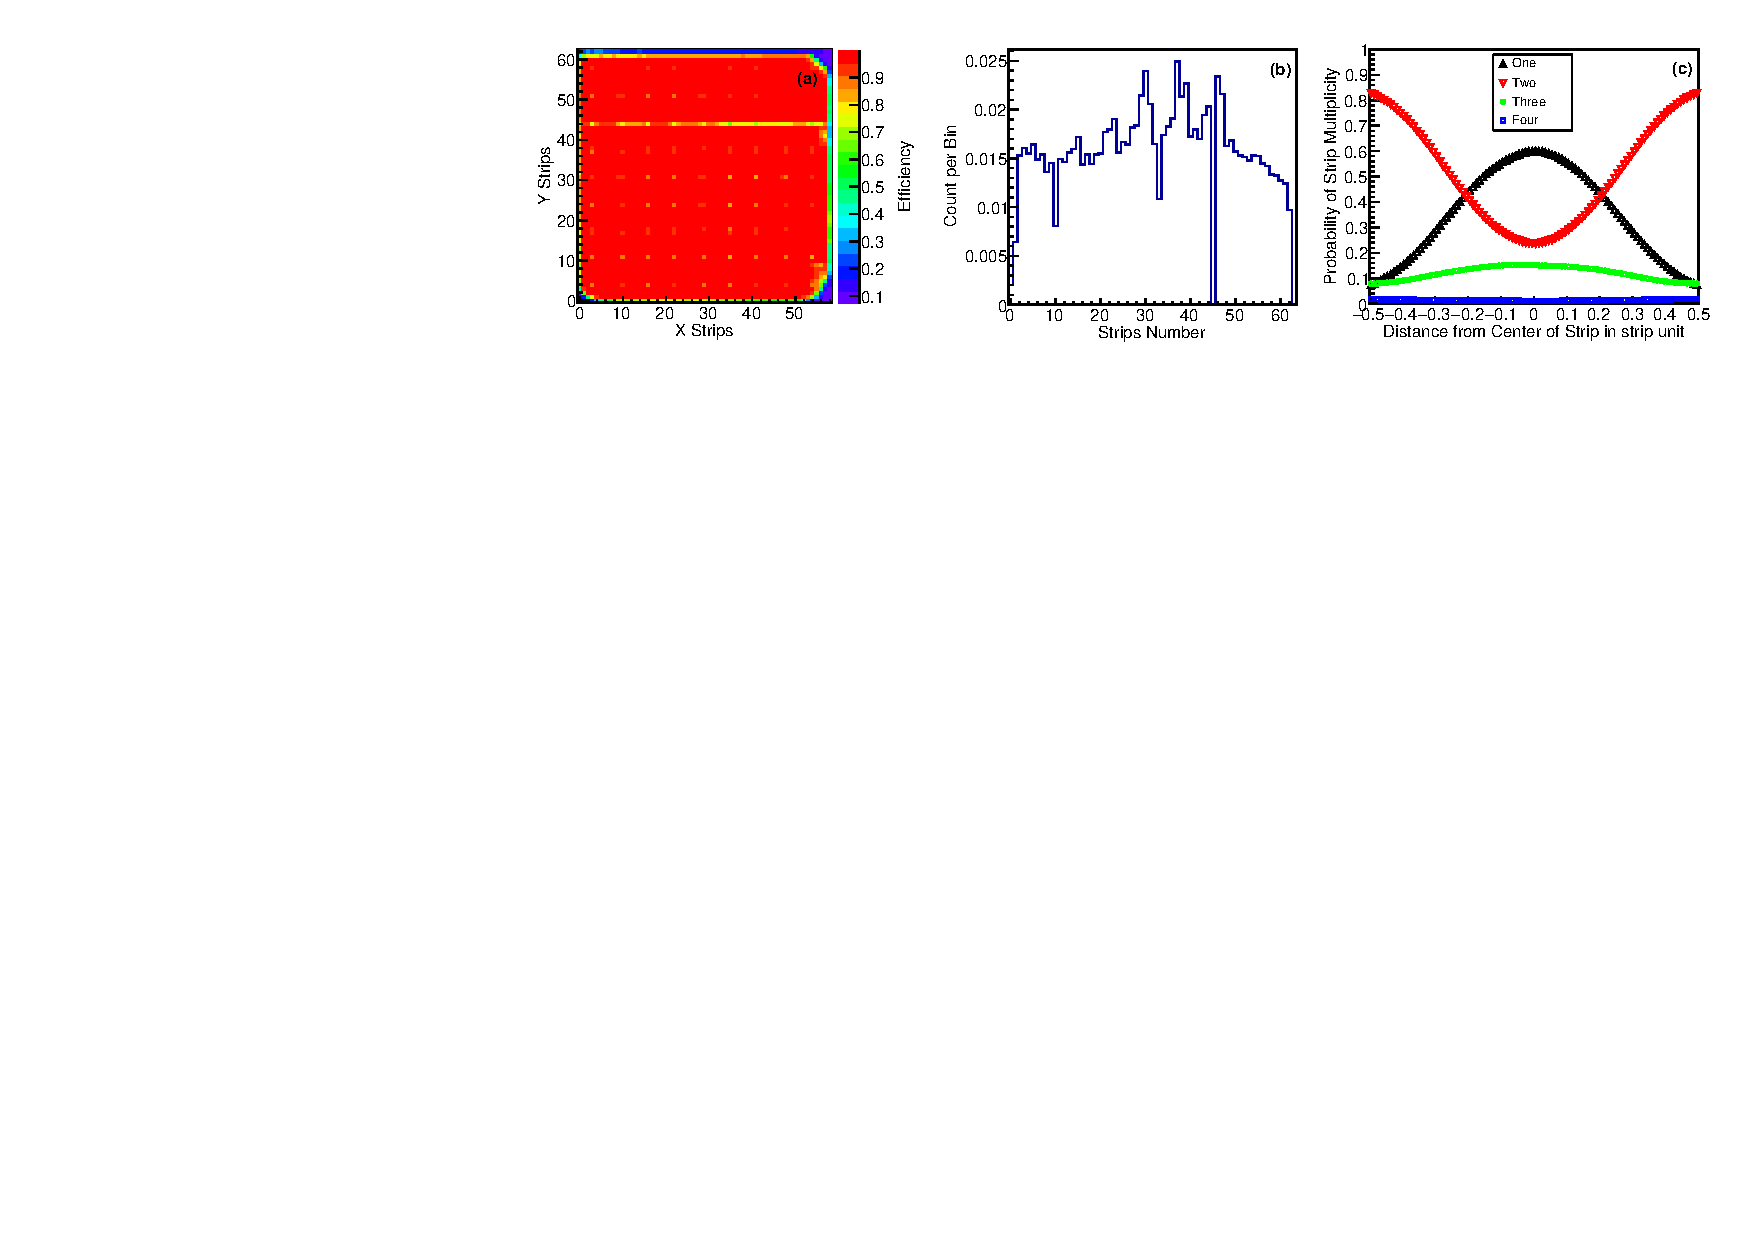
\includegraphics[width=1.\linewidth]{layer2properties.pdf} 
  \caption{(a) Efficiency, (b) Noise and (c) Multiplicity profile of
    Y side of Layer-2 RPC gap.}
  \label{fig:layer2y}
\end{figure}
These observed detector parameters are included in the digitisation
stage of the detector simulation. Both the events from the observed
cosmic ray data and the detector simulation are reconstructed using
an algorithm based on Hough Transformation which is discussed in the
next section.

\section{Event Reconstruction and Data Selection}\label{sec:reconstrction}
During the event reconstruction, the strip hits are analysed
independently, in the 2-dimensional projections namely,
\mbox{X--Z} and \mbox{Y--Z} plane. During the passage of a charged
particle through a RPC gap, the number of strips on which signal is
induced depends on the gain of the gas gap. This sharing of the induced
signal between the neighbouring strips is the main reason for the
observed strip multiplicity shown in the Figure~\ref{fig:layer2y}(c).
In order to prepare the events for analysis, the consecutive strips
which have recorded signal are clubbed together to form a cluster.
During the study, the position resolution is calculated for different
strip multiplicities of 1, 2, 3, and 4 and the values observed are
$\sim$6\,mm, $\sim$8\,mm, $\sim$12\,mm and $\sim$22\,mm respectively.
The position resolutions for strip multiplicities more than four is
larger than the pitch of the strip (3\,cm). So in this study,
the clusters of hits with more than 4 multiplicities are neglected
as the position resolution for higher multiplicities is found to be
the worse. A layer which has more than 15 strip hits and/or more
than 10 clusters is tagged as `noisy layer' and not considered
in the track reconstruction. An event which has more than 3 noisy
layers is considered as `noisy event' and discarded.

In the first step of track reconstruction, the clusters associated
with different tracks are found and grouped using the method of Hough
Transformation\cite{hought}. The equation of the straight line,
used to find the association between the hits, is given as,
\begin{equation}
  r=z\cos\theta+x\left(/y\right)\sin\theta. \label{eq:hough}
\end{equation}
The \mbox{$r$-$\theta$} plane (also called as Hough Space) is
populated using the concept of Cellular Automaton\cite{cellular}.
For a sample event shown in the Figure~\ref{fig:houghPl}(a),
the populated \mbox{$r$-$\theta$} plane is presented in the
Figure~\ref{fig:houghPl}(b).
\begin{figure}[h]
  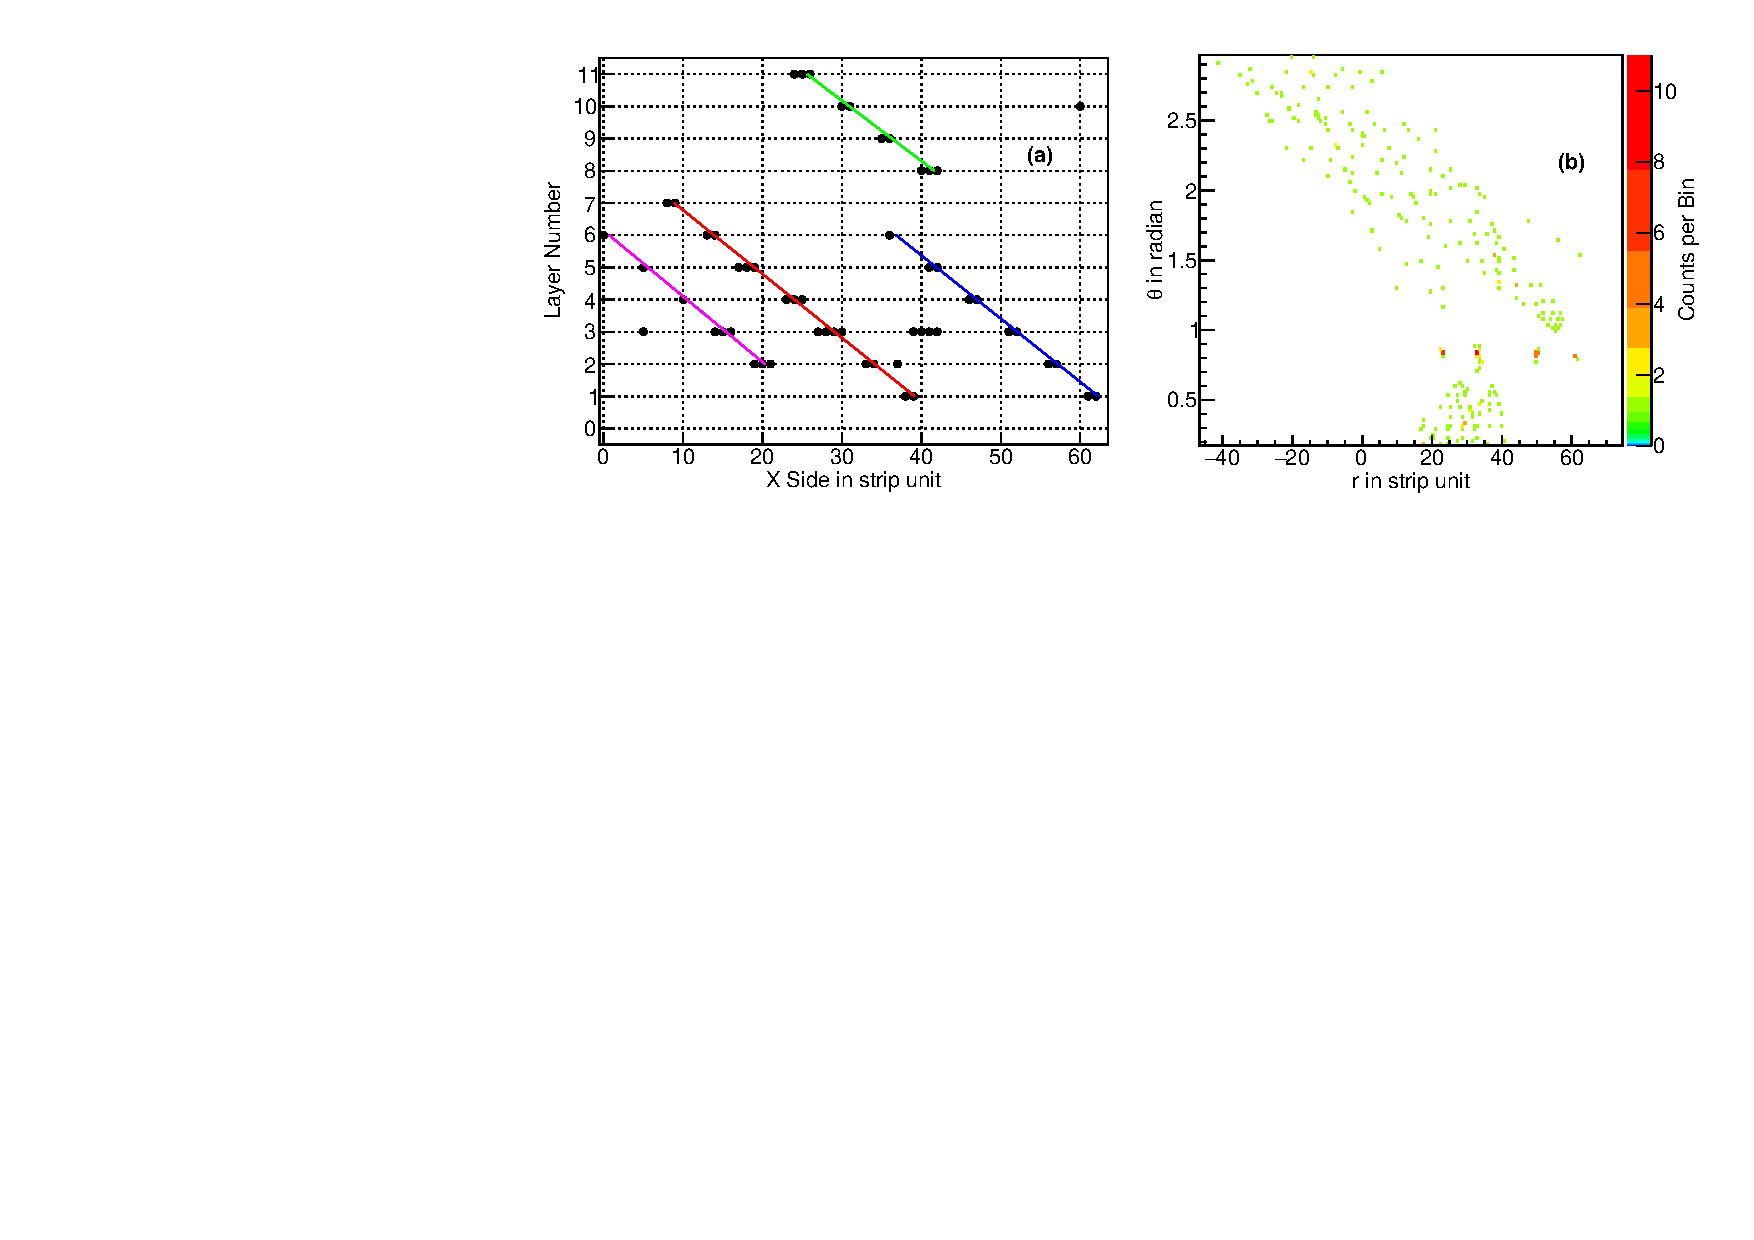
\includegraphics[width=1.0\linewidth]{hough_Plane.pdf} 
  \caption{(a) Projection of an event in the detector and
    (b) populated $r$-$\theta$~plane using this event.}
  \label{fig:houghPl}
\end{figure}
The advantage of using Cellular Automaton technique is the significant
reduction of computation time to find a trajectory in the event.
This method can detect all the tracks avoiding the noise hits as
shown in Figure~\ref{fig:houghPl}(a).

The tracks are identified using the Hough Transformation are then
fitted by a straight line given by the equation,
\begin{equation}
  x\left(/y\right)=mz+c \label{eq:plain}
\end{equation}
where $m$ and $c$ are the slope and the intersect, respectively.
The number of detector layers in the fit and $\chi^{2}$/ndf of
the fit are shown in the Figure~\ref{fig:chi2ndf}(a) and
\ref{fig:chi2ndf}(b) respectively.
\begin{figure}[h]
  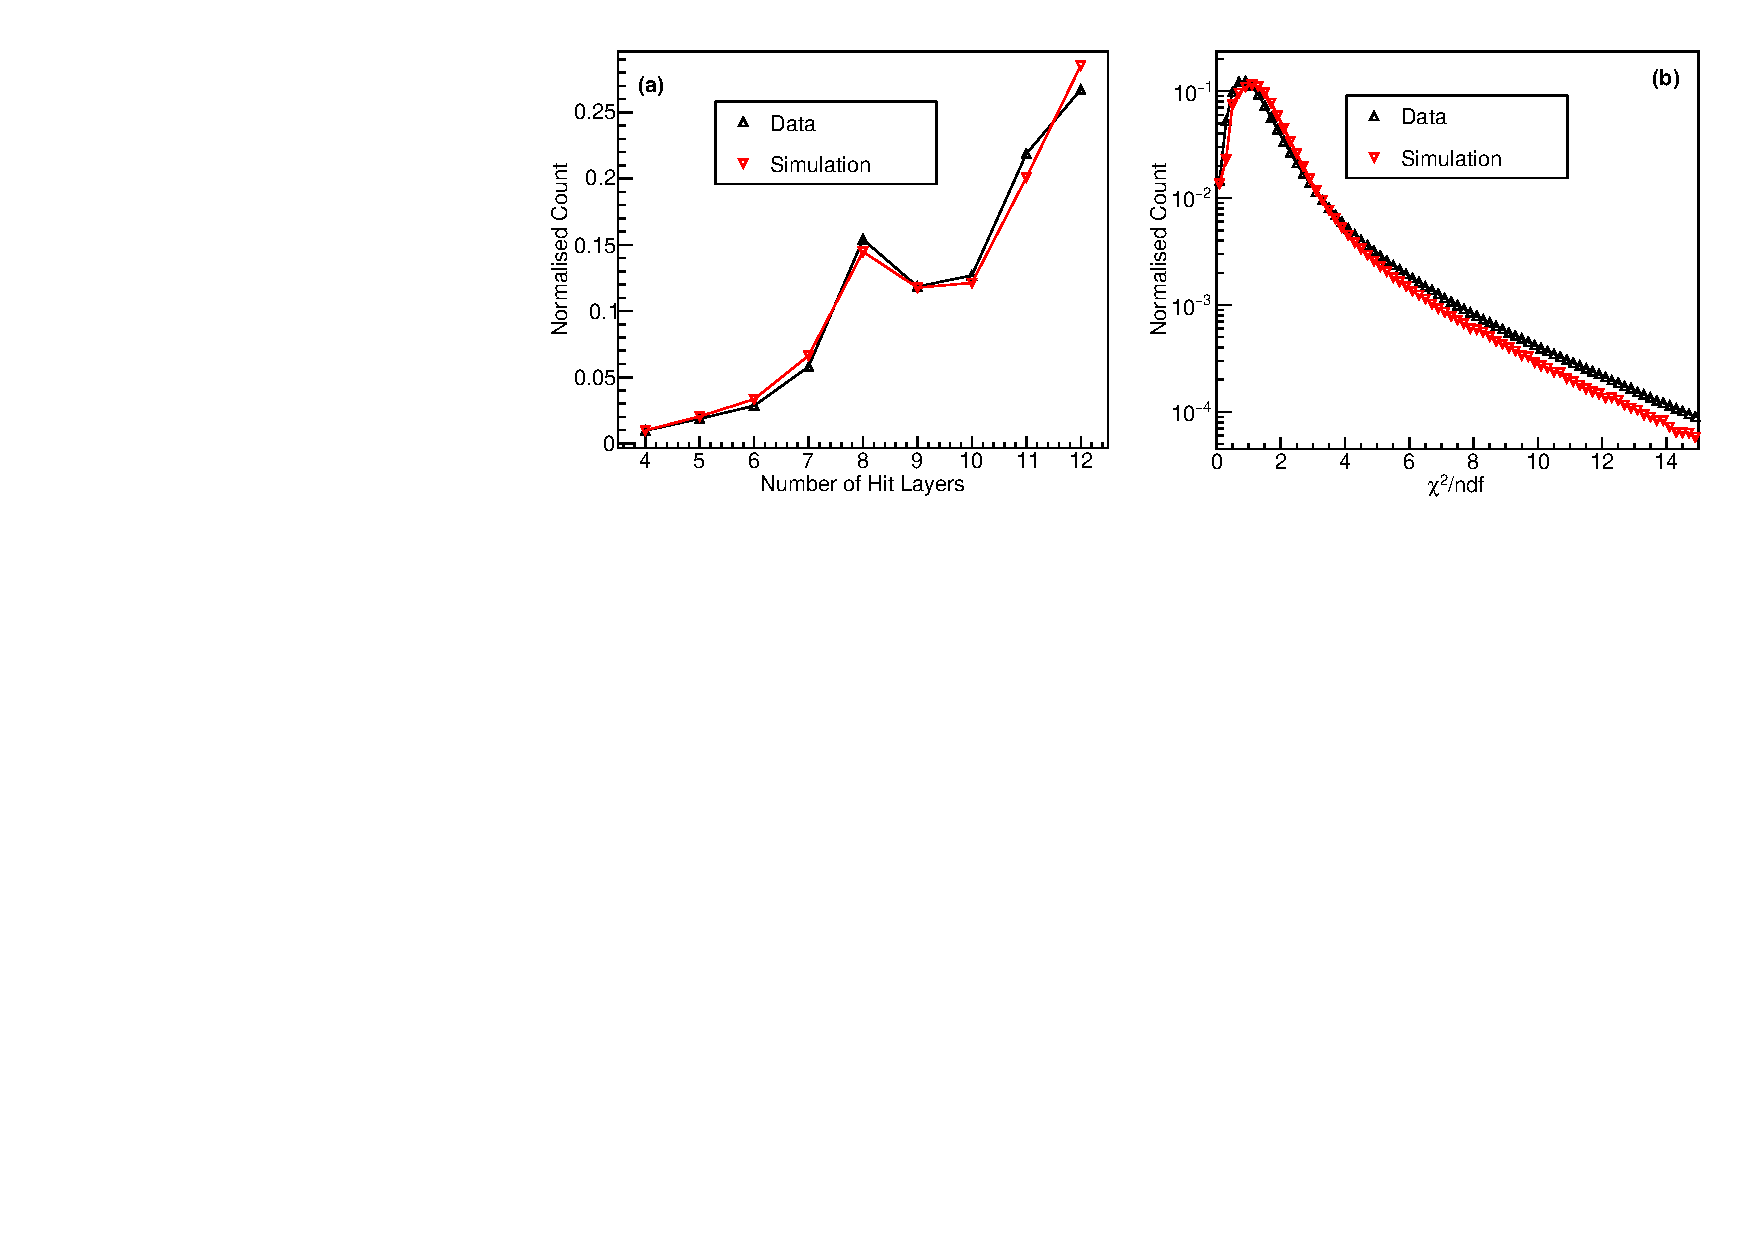
\includegraphics[width=1.0\linewidth]{chi2ndf_compare_all.pdf} 
  \caption{(a) Number of hit layer and
    (b) $\chi^2$/ndf of straight line fit.}
  \label{fig:chi2ndf}
\end{figure}
A track is considered as properly reconstructed if the $\chi^{2}$/ndf
is less than 10 and there are more than 4 layers in the track.
The reconstruction efficiency is defined as the ratio of the number
of events with at-least one reconstructed track to the total number
of triggered events. The reconstruction efficiency as a function of 
time is shown in the Figure~\ref{fig:stackineffi}.
\begin{figure}[h]
  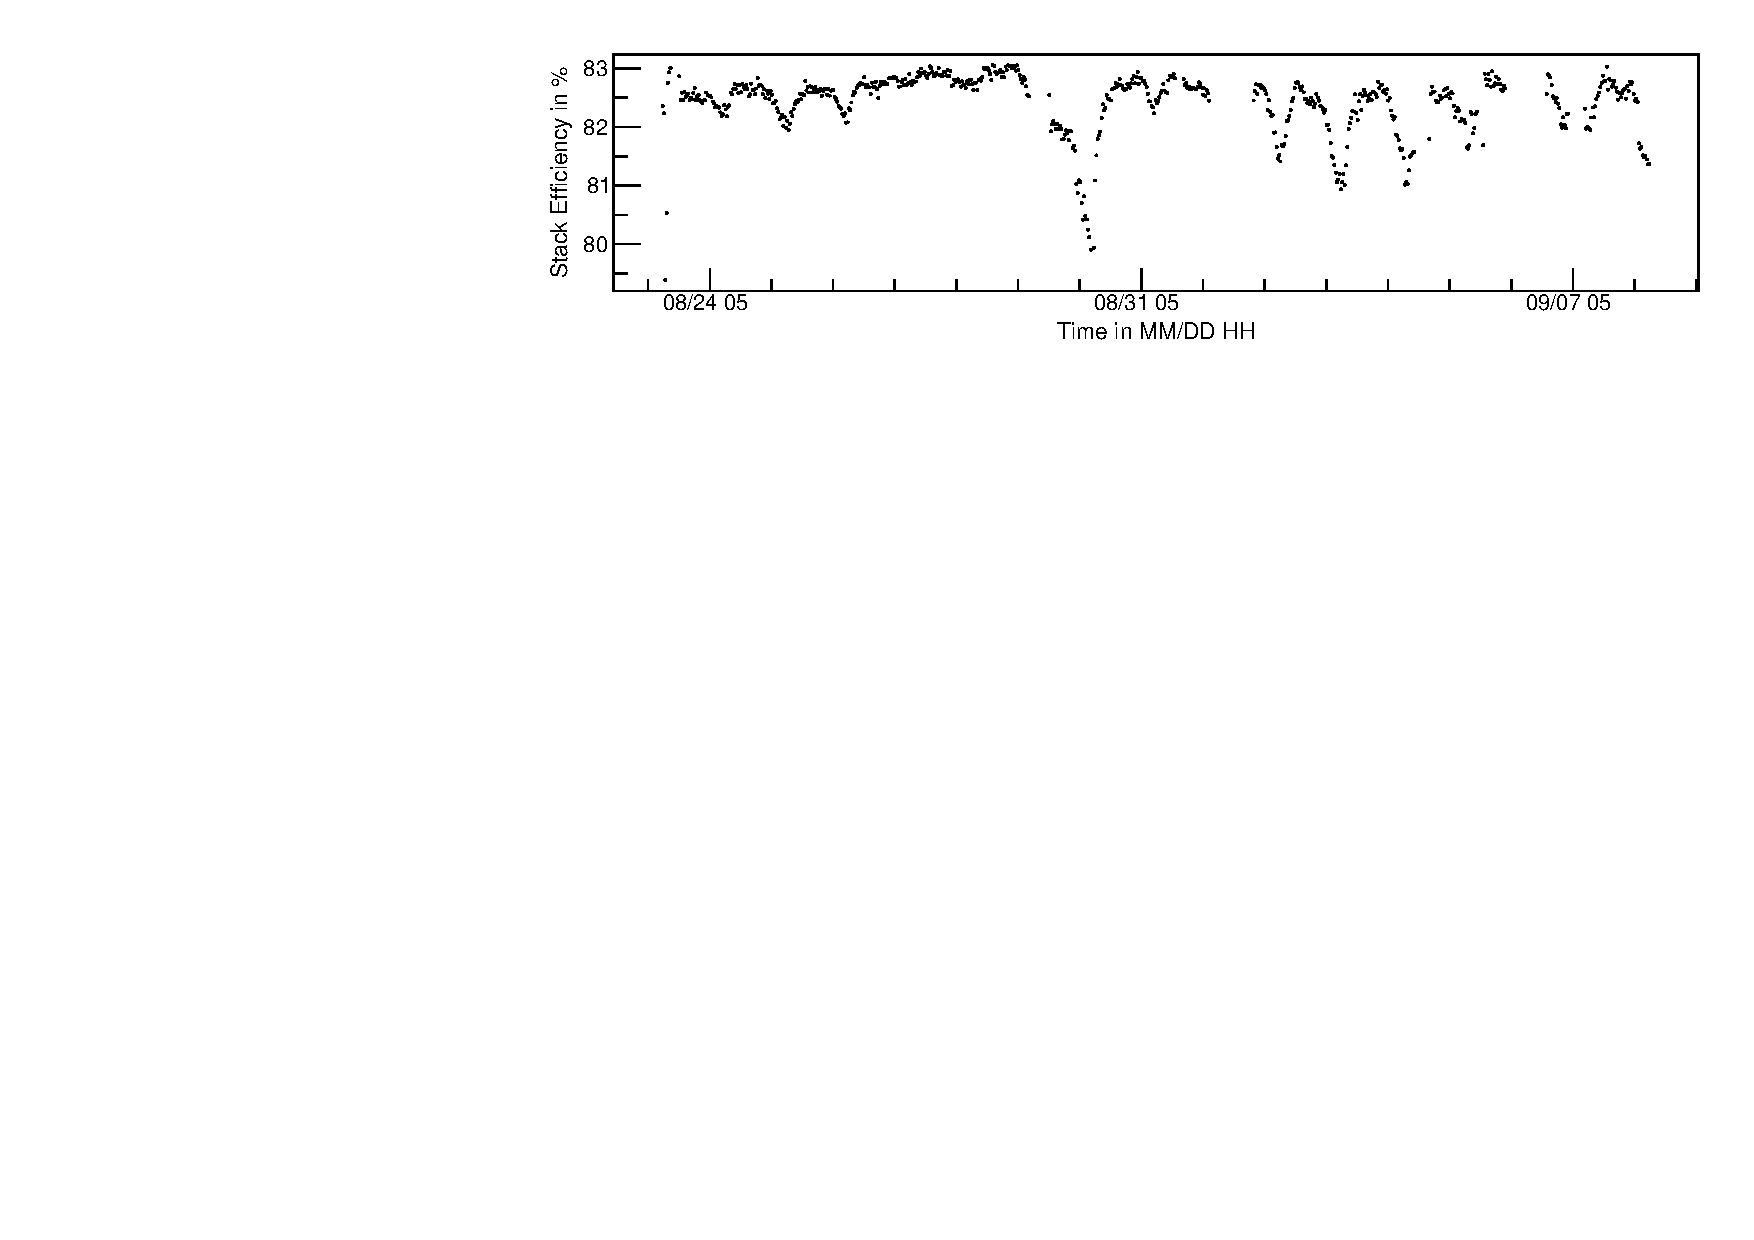
\includegraphics[width=1.0\linewidth]{stack_ineffi_1.pdf} 
  \caption{Variation of reconstruction efficiency of the detector
    with time.}
  \label{fig:stackineffi}
\end{figure}
It can be observed that the reconstruction efficiency varies
periodically with time which is correlated to the variation
of the ambient pressure and temperature. But this periodic change in 
the reconstruction efficiency does not affect the relative ratio of
the multiple track events. The pure multiple track events are
$\sim$0.01\% of triggered events. Out of the total triggered events,
also 6--7\,\% of events are due to noises and hadronic showers
initiated at the roof.
An extreme shower event (which can also be due to the noise) shown
in the Figure~\ref{fig:eshower} can also imitate a multi-track event.
\begin{figure}[h]
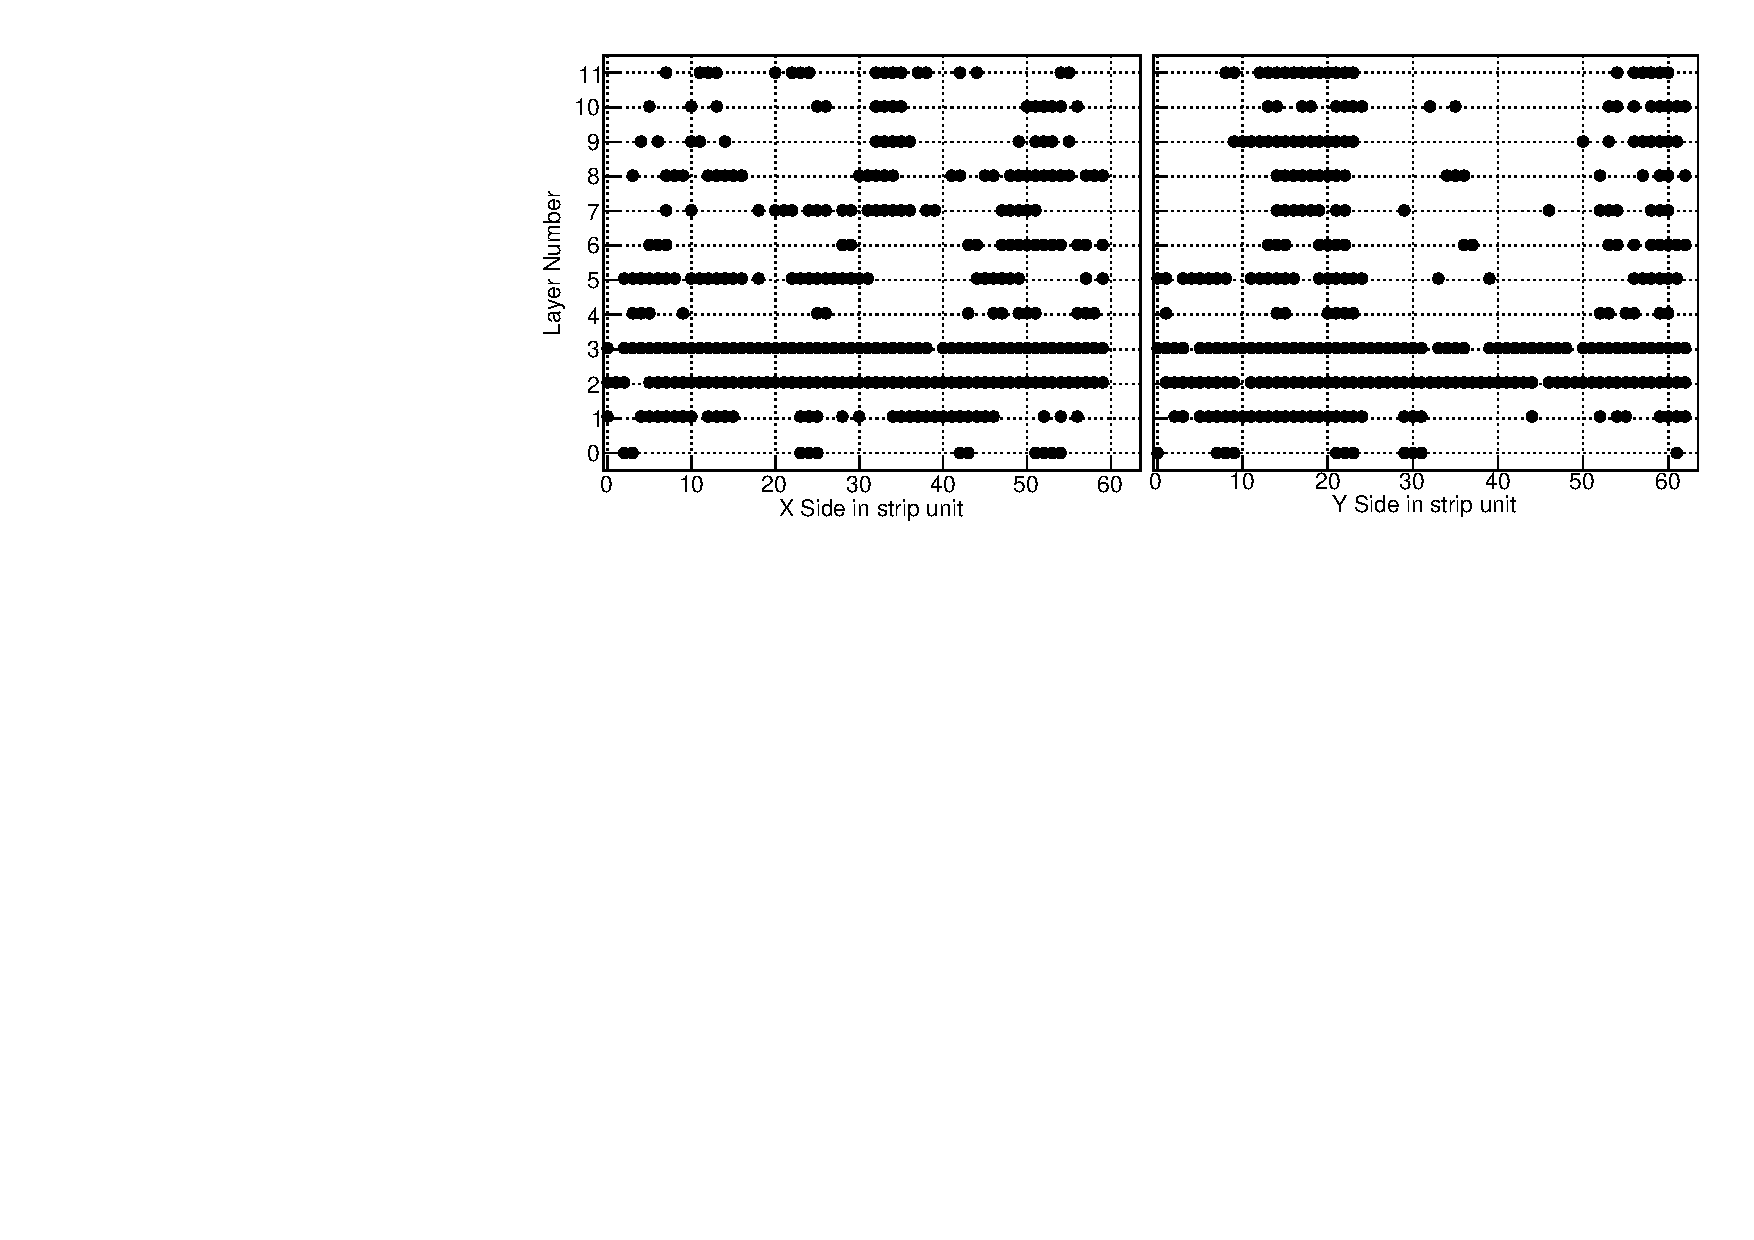
\includegraphics[width=1.0\linewidth]{Multi_Event_20170823_102605_3088_Shower_1.pdf} 
 \caption{Example of an extreme shower event.}
 \label{fig:eshower}
\end{figure}
Any such ambiguous events are rejected by the selection criteria
used in the analysis discussed in the following.

The zenith and azimuthal angle distributions of the reconstructed
tracks are presented in the Figure \ref{fig:thetaphi}(a) and
\ref{fig:thetaphi}(b), respectively.
\begin{figure}[h]
  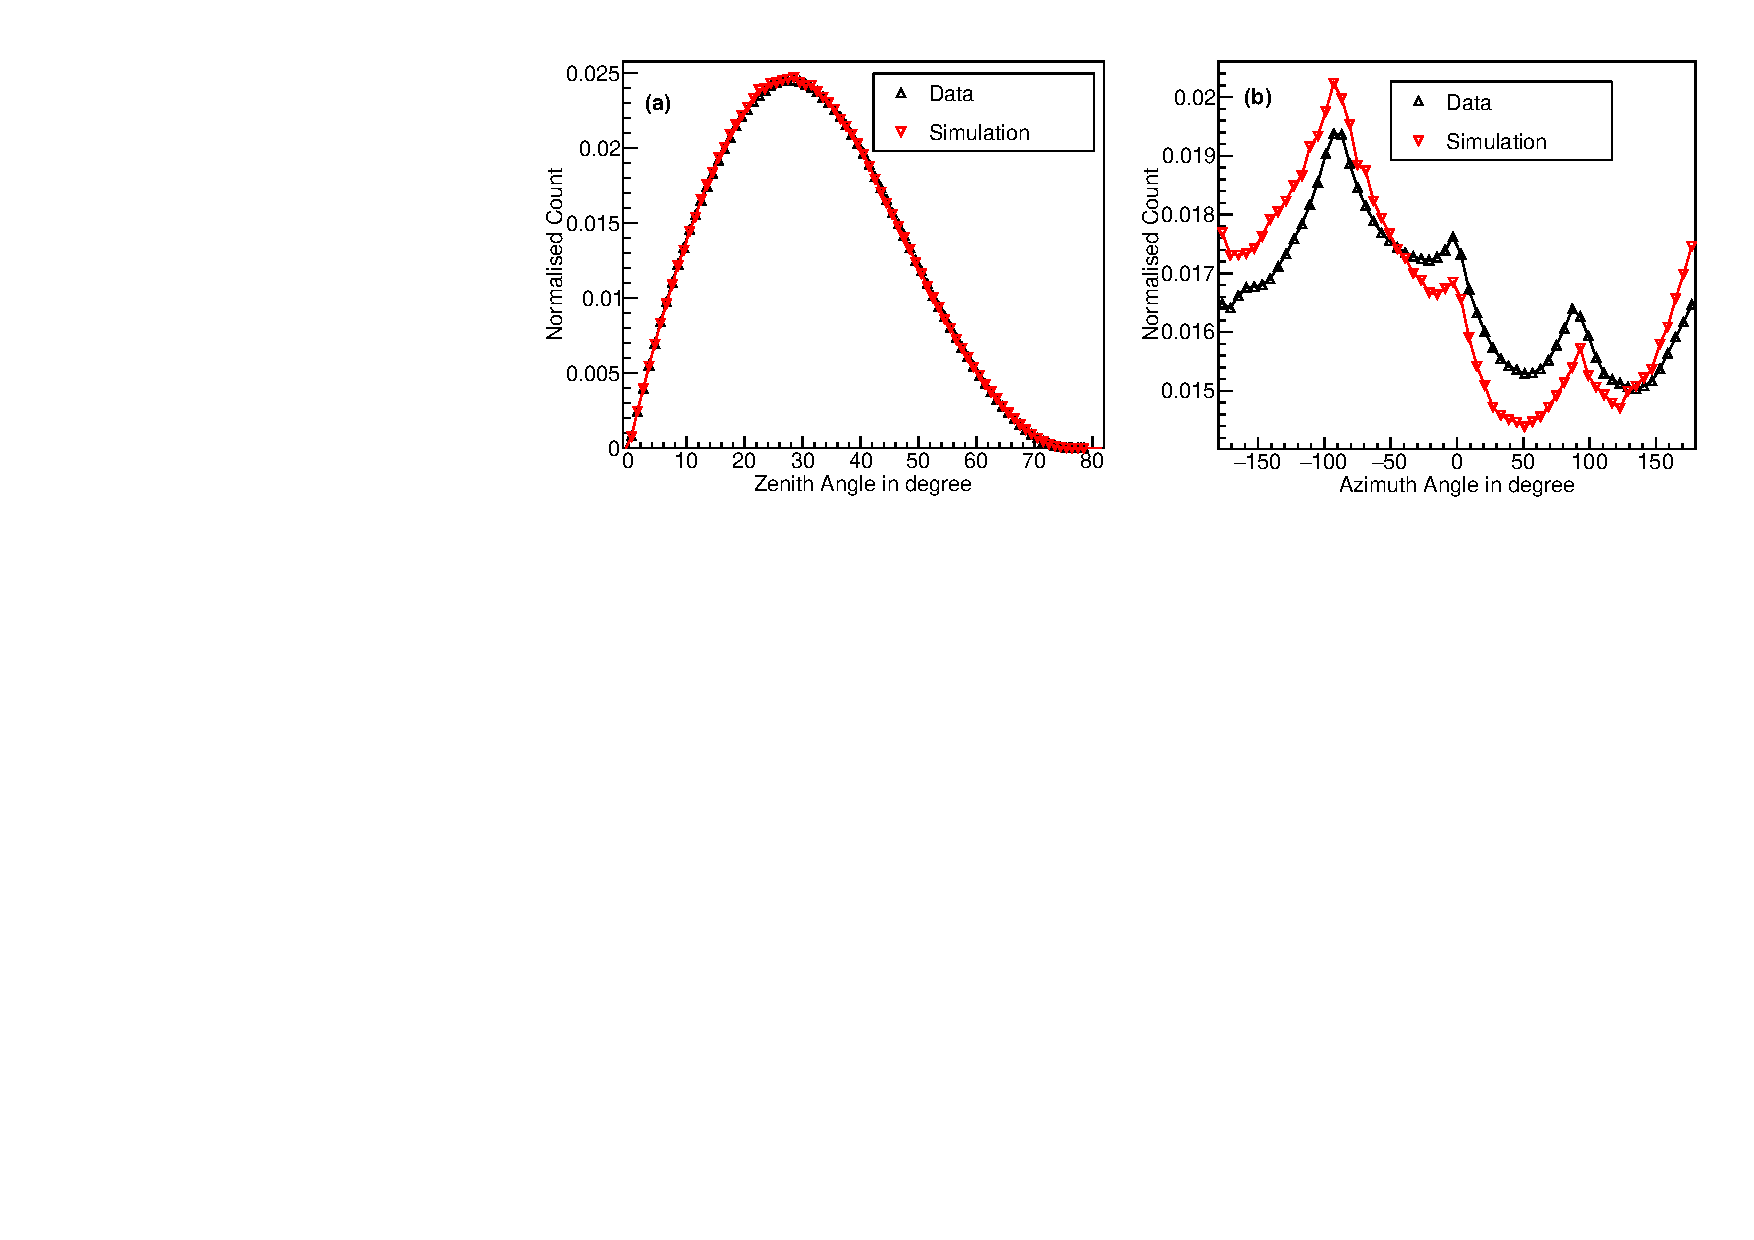
\includegraphics[width=1.0\linewidth]{thetaphi_compare_all.pdf} 
  \caption{(a) Zenith and (b) Azimuth Angle of cosmic rays
    reaching the detector 
stack.}
  \label{fig:thetaphi}
\end{figure}
The projections from both the X--Z and Y--Z planes are combined
to produce final 3-dimensional track(s). Any ghost tracks formed
while combining are discarded by using the timing information recorded
for each strip. The events of interest for this analysis are the
events with more than one reconstructed 3-dimensional track.
The distribution of the time separation between each pair of
reconstructed tracks for both the simulation and data are shown in the
Figure~\ref{fig:time_sep}(a).
\begin{figure}[h]
  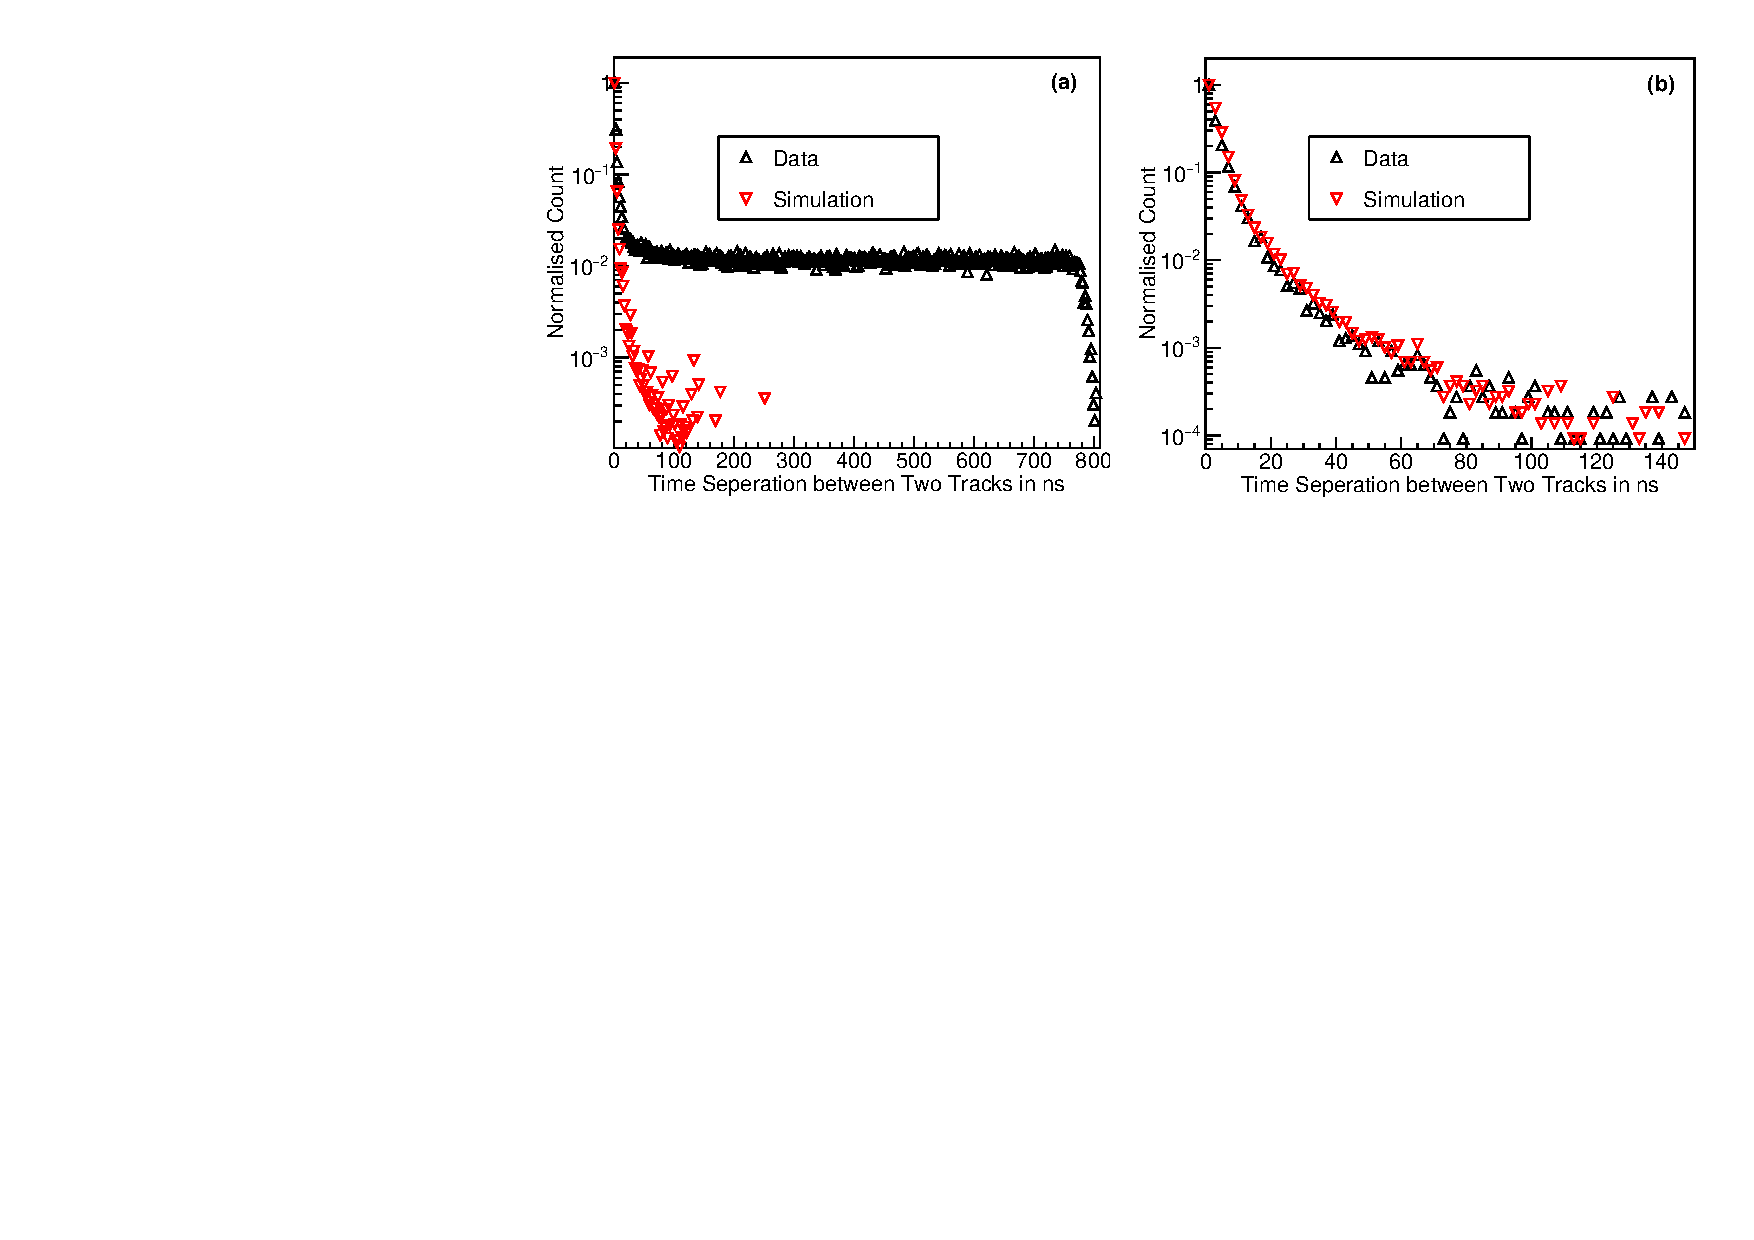
\includegraphics[width=1.0\linewidth]{time_diff_compare_all.pdf} 
  \caption{Time separation of two tracks for (a) all events and
    (b) for events with only parallel tracks.}
  \label{fig:time_sep}
\end{figure}
In the case of data, it can be observed that there is a significant
number of events where multiple particles are reaching the detector
with large relative time delay. The random coincidence of particles
originating in the different cosmic showers is the cause for these
events. The random coincidence of particles from different cosmic
showers are absent in the simulation as only one shower is simulated
at a time in the CORSIKA.

In the simulation, it is observed that the particles originating
from the same shower are detected in the RPC stack as parallel tracks.
This can be verified by calculating the skewed angle between
the two tracks. The skewed angle between two parallel tracks is
ideally supposed to be zero, but due to the finite size of the strip
width and multiple scatterings, it has finite width and tails.
The distribution of the skewed angle between each pair of tracks
for both simulation and data is shown in the
Figure~\ref{fig:skewed_angle}(a).
\begin{figure}[h]
  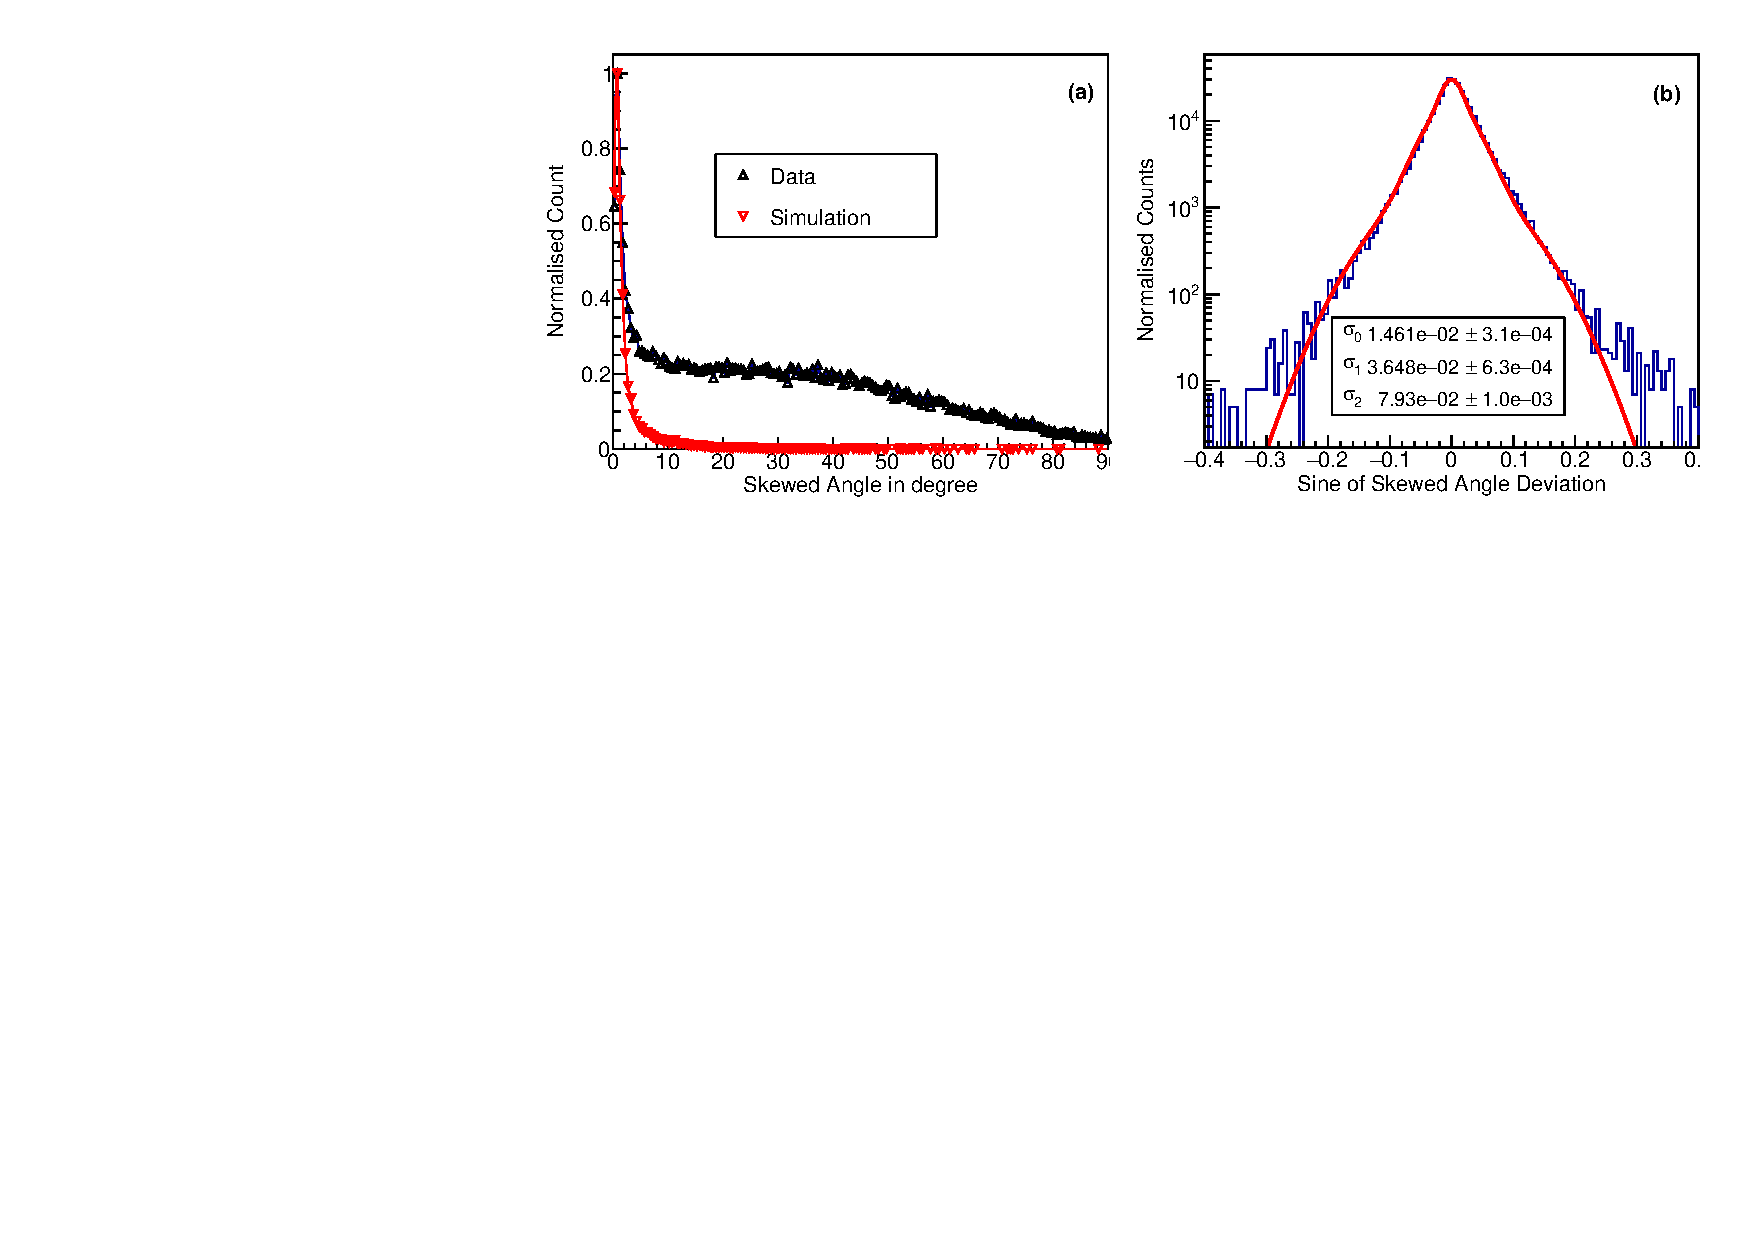
\includegraphics[width=1.0\linewidth]{skewed_compare_reso_2plot_full.pdf}
  \caption{(a) Skewed angle between two tracks originating
    outside of the detector, (b) Skewed angle difference
    between generated and reconstructed tracks fitted with
    triple-gaussian function.}
  \label{fig:skewed_angle}
\end{figure}
In order to understand the application of the skewed angle, events
with multiple particles are simulated in the GEANT4. The distribution
of the sine of the difference of the skewed angle between
the generated particles and the skewed angle between
the reconstructed tracks are shown in the
Figure~\ref{fig:skewed_angle}(b). This distribution is fitted with
a triple-Gaussian function. The three components of these angular
resolutions represent the cases, which are due to no multiple
scattering, one track has large multiple scattering and both
have large multiple scattering.

Based on these observations, the tracks with a skewed angle less than
$\sim 2.5^{\circ}$ are considered as parallel to each other.
Thus, in the current study, only the parallel tracks which are
satisfying the skewed angle cut are considered to be generated
from the particles originating from the same cosmic ray shower.
The time difference between a pair of tracks for both simulated
and observed data after the criteria of parallel track selection
are shown in the Figure~\ref{fig:time_sep}(b). It can be observed
that the events from the random coincidences disappear in the data
after rejecting the events with non-parallel tracks.
